% -*- root: ../modelizacion.tex -*-
\section{Hoja 1}
\begin{problem}[1]
Una \textbf{fuerza central} es una fuerza que en $\overrightarrow{x}$ tiene módulo que sólo depende de $||\overrightarrow{x}||$. Por tanto $\overrightarrow F=m\cdot \overrightarrow a$ lleva a una ecuación del tipo
\[\overrightarrow x '' =g(||\overrightarrow x||)\overrightarrow x\]
Calcula la derivada de $\overrightarrow x\times \overrightarrow  x'$ (el momento angular) y deduce de ello que cada curva solución está contenida en un plano. Otra forma (más complicada) de proceder es probar directamente que la torsión de la curva es nula. Investiga este procedimiento usando la fŕomula de la torsión

\solution
	Definimos la fuerza central (la fuerza que va del origen hasta x) de la siguiente forma:$$\overrightarrow F = g(||\overrightarrow x||) \overrightarrow x$$

	Como $\overrightarrow F = m \cdot \overrightarrow a$ entonces $m\overrightarrow x'' = g(||\overrightarrow x||) \overrightarrow x$\\
	De esto último deducimos que $\overrightarrow x \times \overrightarrow x'' = \overrightarrow 0$ puesto que son vectores paralelos.

	Por lo tanto $\frac{\dif}{\dif t}(\overrightarrow x \times \overrightarrow x') = \overrightarrow x \times \overrightarrow x + \overrightarrow x \times \overrightarrow x '' = \overrightarrow 0 + \overrightarrow 0.$

	Y con esto ya tenemos que $\overrightarrow x $ está en un plano ya que:

	$$\overrightarrow x \times \overrightarrow x' = \overrightarrow V_0 \text{ que es }
	cte \implies \overrightarrow V_0 \cdot \overrightarrow x = 0 \stackrel{V_0 \neq 0}{\implies} \overrightarrow x \text{está en un plano}$$
	¿Qué ocurriría con $V_0 = 0$?

	$x'$ y $x$ serían paralelos, es decir, la velocidad iría en la dirección de x $\implies$ $\overrightarrow x$ está en una recta.

	La explicación de la última implicación se deja como ejercicio.

	Otra forma de ver que $\overrightarrow x$ está en un plano es utilizando la torsión:

	Definimos la curva
	\[t \mapsto \overrightarrow{x(t)}\]
	y la torsión
	\[T = \frac{(\overrightarrow x' \times \overrightarrow x'') \cdot \overrightarrow x'''}{||\overrightarrow x' \times \overrightarrow x ''||}\]

	Por la fórmula de la $\overrightarrow F$ puesdo escribir:
	$$\overrightarrow x'' = \frac{1}{m} g(||\overrightarrow x||)\overrightarrow x $$

	Y si dervivamos:

	$$\overrightarrow x''' = \frac{1}{m} g'(||\overrightarrow x||) \frac{\overrightarrow x \cdot \overrightarrow x'}{||\overrightarrow x||} \overrightarrow x + \frac{1}{m}g(||\overrightarrow x||)\overrightarrow x' = \frac{g'(||\overrightarrow x||)}{g(||\overrightarrow x||)}\cdot \frac{\overrightarrow x \cdot \overrightarrow x'}{||\overrightarrow x||} \overrightarrow x'' + \frac{1}{2}g(||\overrightarrow x||) \overrightarrow x''$$

	Con esto podemos ver que $\overrightarrow x'''$ es combinación lineal de $\overrightarrow x''$ y $\overrightarrow x'$ y por tanto:
	$$(\overrightarrow x' \times \overrightarrow x'' \times \overrightarrow x''') = det(\overrightarrow x', \overrightarrow x'',\overrightarrow x''') = 0 \stackrel{\implies}{\overrightarrow x' \times \overrightarrow x'' \neq 0} T = 0 \implies \text{curva plana}$$
\end{problem}

\begin{problem}[2]

La estación espacial internacional orbita a unos 400 km de la superficie dela Tierra. Calcula en qué proporción ha disminuido la fuerza de la gravedad a esa altura. ¿Cuánto pesaría una persona de 80kg a esa altura? ¿Por qué entonces las imágenesque nos llegan muestran astronautas y objetos flotando ingrávidos?

\solution
	Queremos ver el peso de una persona a 400 km de la Tierra

	Llamamos M a la masa de la tierra; m, al peso de una persona y R, al radio de la Tierra.

	Vemos la relación entre la fuerza que hay sobre la persona en la superficie de la Tierra y la fuerza a 400 km:

	$$\frac{\frac{GMm}{R^2}}{\frac{GMm}{(R + 400000 m)^2}} \implies \frac{(R + 4\cdot 10^5)^2}{R^2} = \left(\frac{67.8}{63.8}\right)^2$$

	Por lo tanto, si m = 80, el peso a 400 km sería:
	$$\frac{80}{\left(\frac{67.8}{63.8}\right)^2} = 70 .84 Kg$$

	\textbf{Pregunta del profesor:} Los astronautas están flotando alrededor de la Tierra por la fza.centrífuga. ¿Porqué no ocurre lo mismo en la superficie?
\end{problem}

\begin{problem}[3]
Prueba que la curva en polares $r(\theta)= \frac{a^{-1} \cdot b^2}{1 + e\cos\theta}$ siendo
\[ e = \frac{c}{a} = \sqrt{1 - \frac{b^2}{a^2}}\]
describe la elipse $\frac{x^2}{a^2} + \frac{y^2}{b^2} = 1$ cuando el origen de las coordenadas polares está en uno de los focos.

Prueba también que la curva en polares
\[r(\theta)=\frac{l}{1+e\cos(\theta)}\]
con $e \geq 0$ y $l>0$ constantes, describe una circunferencia si $e=0$, una elipse si $0<e<1$, una parábola si $e=1$ y una hipérbola si $e>1$.

\textbf{Indicación:} Escribe $r(1+e\cos(\theta)$ en cartesianas.

\solution

    Tenemos la elipse expresada en polares:$$r(\theta)= \frac{a^{-1} \cdot b^2}{1 + e\cos\theta} \text{  siendo  } e = \frac{c}{a} = \sqrt{1 - \frac{b^2}{a^2}}$$

    Y queremos llegar a: $$\frac{x^2}{a^2} + \frac{y^2}{b^2} = 1$$

    Esto es la elipse en cartesianas cuando el origen está en uno de sus focos. Como es lógico buscamos el cambio a cartesianas y para ello reescribimos la ecuación:

    $$ r + er\cos\theta = a^{-1} b^2 \text{ con }
    \begin{cases}
    r = \sqrt{x^2 + y^2}\\
    r\cos\theta = x\\
    \end{cases}$$

    Despejando y elevando al cuadrado en ambos lados obtenemos:
    \[(\sqrt{x^2 + y^2})^2 = (a^{-1}b^2 - ex)^2 \implies x^2 + y^2 = a^{-2} b^4 + e^2x^2 - 2a^{-1}b^2ex\]

    Agrupamos los términos:

    \[(1-e^2)x^2 + y^2 = a^{-2} b^4 - 2a^{-1}b^2ex\]


    Como $1-e^2 = \frac{b^2}{a^2}$ tenemos que

    $$\frac{x^2}{a^2}b^2 + y^2 = a^{-2} b^4 - 2a^{-1}b^2ex$$

    Viendo en la fórmula final el término $\frac{y^2}{b^2}$, dividimos por $b^2$ en ambos lados de la ecuación y completamos cuadrados para $x$ obteniendo:
    $$\frac{(x + a\cdot e)^2}{a^2} + \frac{y^2}{b^2} = 1$$

    Este resultado sería el que nos piden si $e$ vale cero ($a>0$), en cuyo caso es exactamente una circunferencia y el centro coincide con "los focos" tal y como se indica en el enunciado.
\end{problem}

\begin{problem}[4]
Sea $V$ el potencial de una fuerza $\overrightarrow F$, esto es $\overrightarrow F = -\nabla V$, que satisface div$\overrightarrow F = 0$. Demuestra que si $V$ es una función radial (sólo depende de la distancia al origen), entonces necesariamente $\overrightarrow F=K||\overrightarrow x||^{-3}\overrightarrow x$, como con la ley de gravitación universal

\solution
\textcolor{blue}{Hecho por De Juan. No fiarse al 100\%}

Podemos descomponer el potencial en una composición de 2 funciones:

$\appl{d}{ℝ^3}{ℝ}$, con $d(x,y,z) = \norm{\overrightarrow{x}}$.

$\appl{f}{ℝ}{ℝ}$.

Con esta construcción, para alguna $f$ tenemos $V(\vx) = f(d(\vx))$.

Si logramos demostrar que $f$ tiene que ser de la forma $f(x) = \frac{-KM}{x}$, ya tendremos el ejercicio hecho puesto que su gradiente nos daría una fuerzo con fórmula como la indicada.

Ahora sólo hay que derivar con cuidado:

$$-\overrightarrow{F} = \grad V(\vx) = f'(d(\vx)) · \grad d(\vx) = f'\left(\norm{\vx}\right)\frac{1}{\norm{\vx}} \vx$$

\obs Hay que prestar especial atención al hecho de que al escribir $\vx$ hacemos referencia a un vector y no a una variable.

Vemos que $\appl{F}{ℝ^3}{ℝ^3}$. Calculamos la divergencia de $\overrightarrow{F}$

$$div \overrightarrow{F} = \frac{\partial{F}}{\partial{x}} + \frac{\partial{F}}{\partial{y}} + \frac{\partial{F}}{\partial{z}}
\overset{hip.}{=} 0$$


Basándonos en la expresión de la fuerza calculada anteriormente tenemos:

$$\frac{\partial{F(\vx)}}{\partial{x}} = \left(\underbrace{\dpa{f'(d(\vx))}{x}}_{(1)} · d(\vx) - f'(d(\vx))\dpa{d(\vx)}{x} \right)\frac{x}{(d(\vx))^2} + \frac{f'(d(\vx))}{d(\vx)}$$

$(1) = \dpa{d(\vx)}{x} · f''(d(\vx))$ por la regla de la cadena.

Simplificando y utilizando el cálculo anterior, obtenemos:

$$\dpa{F(\vx)}{x} = \frac{x^2}{(d(\vx))^3}\left(f''(d(\vx)) d(\vx) - f'(d(\vx))\right) + \frac{f'(\vx)}{d(\vx)}$$

El cálculo es análogo para las derivadas respecto de $y,z$, con lo que la divergencia queda:

$$div \overrightarrow{F} = \left(f''(d(\vx)) d(\vx) - f'(d(\vx))\right) \cdot \frac{x^2 + y^2 + z^2}{(d(\vx))^3} + \frac{3f'(d(\vx))}{d(\vx)}$$

Tomamos $d(\vx) = r$ y utilizamos $x^2+y^2+z^2 = \left(\sqrt{x^2+y^2+z^2}\right)^2 = d(\vx)^2$

$$ div \overrightarrow{F} = 0 = \left((f''(r)r - f'(r)) + 3f'(r)\right) \frac{1}{r} = 0 \dimplies r f''(r) = -2 f'(r)$$

Hemos llegado a una EDO cuya solución es $g(x) = \frac{k}{x}$, porque:

$$g(x) = \frac{k}{x} \implies g'(x) = \frac{-k}{x^2} \implies g''(x) = \frac{2k}{x^3}$$

Vemos que $x g''(x) = x\frac{2K}{x^3} = \frac{2K}{x^2} = -2 \frac{-K}{x^2} = -2 g'(x)$ que es la EDO que teníamos.

Por tanto ya tenemos el ejercicio resuleto, pues la $f$ obtenida coincide exactamente con lo que esperábamos obtener. Veamos por que está $f$ garantiza la fórmula para la fuerza que indica el enunciado.
$$V(\vx) = f(d(\vx)) = \frac{K}{d(\vx)} = \frac{K}{\norm{\vx}}$$

Y para hallar la $\overrightarrow{F}$, utilizamos $$\overrightarrow{F} = - \grad V = -K\left(\frac{-x}{\norm{\vx}^{3}},\frac{-y}{\norm{\vx}^{3}},\frac{-z}{\norm{\vx}^{3}} \right)$$

Y reescribimos : $$\overrightarrow{F} = - \grad V = \frac{K}{\norm{\vx}^3} \vx$$

\end{problem}

\begin{problem}[5]
Explica por qué en el punto más cercano al Sol de la órbita de una planeta, digamos a distancia $r_p$, la velocidad $v_p$ debe cumplir $v_p=r_p\theta'$. Recuerda que en el movimiento de un planeta $h=r^2\theta'$ es constante y que $a(1-e^2)=h^2/GM$ con $a$ el semieje mayor y  $e$ la excentricidad. Deduce de todo ello que $v_p=br^{-1}_p\sqrt{GM/a}$

\solution
Para probar que $v_p=r_p\dot{\theta}$ recordamos que estamos tomando $v_p = ||\overrightarrow v||_p$.

Cogemos la fórmula general de $v$ : $$ v = ||(\dot{x}, \dot{y})|| \implies v= \sqrt{\dot{x}^2 + \dot{y}^2}$$
Hacemos el cambio de variables
$\begin{cases}
x = r\cos\theta\\
y = r\sin\theta
\end{cases}$ de forma que
$$v = \sqrt{\dot{r}^2 + r^2\dot{\theta}^2}$$
Como en el punto más cercano al sol la distancia alcanza un mínimo $\implies \dot r = 0$, entonces
$$v= r\dot{\theta} \implies v_p = r_p\dot{\theta}$$

Ahora vamos a deducir:
\[v_p = \frac{b}{r_p}\cdot \sqrt{\frac{GM}{a}}\]

Por el enunciado sabemos que
$$v_p = \frac{h}{r_p} = \frac{\sqrt{GMa(1-e^2)}}{r_p}$$
Solo nos queda probar que $\sqrt{a(1-e^2)}= \frac{b}{\sqrt{a}}$ , o l que es lo mismo
$$a(1-e^2) = \frac{b^2}{a}$$
Utilizamos la relación de la excentricidad (e) con los semiejes (a,b).

Sabemos que $e = \frac{c}{a}$, siendo c la distancia focal $\implies c= \sqrt{a^2-b^2}$ entonces $e = \frac{\sqrt{a^2 - b^2}}{a}$.

Sustituyendo:
$$a(1-e^2) = \frac{b^2}{a} \implies a(1-\frac{a^2 - b^2}{a^2}) = \frac{b^2}{a}$$
Vemos que es cierto, por lo tanto $v_p = \frac{b}{r_p}\cdot \sqrt{\frac{GM}{a}}$
%Esto lo comento por que creo que no vale para nada, pero me da pena tirarlo por si acaso
%Por el principio básico de la mecánica (principio de Hamilton) sabemos que la trayectoria del sistema da un extremo de
%\[\int_{t_0}^T L = \int_{t_0}^T E_{cinetica}-E_{potencial} = \int_{t_0}^T \frac{1}{2}mv^2-\frac{GMm}{r}\]
%Sabiendo que la velocidad es la derivada de la posición y que las órbitas son planas podemos escribir:
%\[\int_{t_0}^T L = \int_{t_0}^T \frac{1}{2}m\left(\dot{x}^2+\dot{y}^2\right)-\frac{GMm}{\sqrt{x^2+y^2}}\]
%Puesto que no depende de $t$ tenemos que la energía es constante. Es decir:
%\[E = \dot{x}\frac{\partial L}{\partial \dot{x}}+\dot{y}\frac{\partial L}{\partial \dot{y}}-\frac{1}{2}m\left(\dot{x}^2+\dot{y}^2\right)-\frac{GMm}{\sqrt{x^2+y^2}} = cte\]
%Vamos a trabajar esta ecaución a fin de llegar al resultado buscado:
%\[\dot{x}\dot{x}'+\dot{y}\dot{y}'-\frac{1}{2}\left(\dot{x}^2+\dot{y}^2\right)-\frac{GM}{\sqrt{x^2+y^2}} = cte\]
\end{problem}

\begin{problem}[6]
Prueba que si el semieje mayor de la elipse de un planeta es $a$ entonces su velocidad cuando está a distancia $r$ del Sol es $\sqrt{2GM/r-GM/a}$.

\textbf{Indicación:} Utiliza el problema anterior y la conservación de la energía.
\solution
\textbf{Idea:} En $v_p = \frac{b}{r_p}\cdot \sqrt{\frac{GM}{a}}$ (ejercicio anterior) hay información redundante, ya que $b,a\text{ y } r_p$ están relacionadas, no son independientes.

La conservación de la energía me dice que
$$\frac{1}{2}m v^2 - \frac{GMm}{r} \text{ es cte}$$

Como tengo la velocidad en un punto ($v_p$), me queda
$$\frac{1}{2} v^2 - \frac{GM}{r} = \frac{1}{2} v_p^2 - \frac{GM}{r}$$
Entonces
$$v = \sqrt{\frac{2GM}{r} + v_p^2 - \frac{2GM}{r_p}}$$
¿Cómo simplifico esto? mirando lo que queremos demostrar sólo queda probar que:
$$\frac{2GM}{r_p} - v_p^2 = \frac{GM}{a}$$
Sustituimos $v_p$ por lo que teníamos en el ejercicio anterior:
$$\frac{2GM}{r_p} - v_p^2 =\frac{2GM}{r_p} -\frac{GMb^2}{ar_p^2} = \frac{GM}{r_p}\left(2-\frac{b^2}{a r_p}\right) $$
Para que la expresión se parezca más a lo que queremos demostrar pensamos qué relación hay entre $r_p$ y a.


Como $e = \frac{c}{a}$ y $r_p = a-c$, sustituyendo:$$\frac{GM}{a(1-e)} \cdot \left(2-\frac{b^2}{a^2(1 - e)}\right)$$

Para terminar bastaría comprobar que:
$$\frac{1}{(1-e)} \cdot (2- \frac{b^2}{a^2(1-e)}) = 1$$

Es fácil usando las siguientes propiedades:
$$e^2 = \frac{c^2}{a^2} = 1-\frac{b^2}{a^2} \implies b^2 = a^2(1-e^2)$$

Finalmente
$$\frac{1}{1-e} \cdot \left(2 - \frac{1 - e^2}{1 - e}\right) = \frac{1}{1-e} \cdot (2-(1 + e)) = 1$$

Por tanto queda demostrado que
$$\frac{2GM}{r_p} - v_p^2 = \frac{GM}{a}$$

Y ya tenemos sustituyendo en la ecuación inicial que
\[v=\sqrt{\frac{2GM}{r}- \frac{GM}{a}}\]
\end{problem}

\begin{problem}[7]
El cometa Halley tiene distancias máxima y mínima al Sol dadas por $5.25\cdot 10^{12} m$ y por $8.77\cdot10^{10}$ m, respectivamente. Calcula la fórmula de su elipse en coordenadas cartesianas, su valor de $r^2\theta'$ y sus velocidades máxima y mínima.

\solution

\textbf{Solución de clase}

$$ \frac{(x+c)^2}{a^2} + \frac{y^2}{b^2} =  1 \;\;\;\; c = a e $$

$$ \begin{cases}
		a + (1+e) = 5.25 * 10^{12} \\
		a(1-e) = 8.77 * 10^{10}
	\end{cases} \} \Rightarrow \begin{cases}
		a = 2.67 * 10^{12} \\
		e = 0.967
	\end{cases}$$

	Con esto calculamos $c = a e = 2.58 * 10^{12}$ y $b = 6.80 * 10^{11}$

\textbf{b)} clase (ver ej. 5)

$$ \frac{h^2}{GM} = a(1- e^2) \;\;\; h = r^2 \theta' $$
$$ h = r^2 \theta' = \sqrt{GMa(1 - e^2)} = 5.53 * 10^{25} $$

\textbf{c)} $v_{\text{max}}$  $ v_{\text{min}}$

Hay que tener en cuenta que la velocidad máxima se alcanza en el perihelio (punto de la órbita con distancia más corta) y la mínima en el afelio (punto opesto al perihelio).

$$ v_{\text{max}} = \sqrt{\frac{2GM}{a(1-e)} - \frac{GM}{a}} =^{\text{a)}} 5.45 * 10^4 m/s $$

$$ v_{\text{min}} = \sqrt{\frac{2GM}{a(1+e)} - \frac{GM}{a}} =^{\text{a)}} 9.14 * 10^2 m/s $$

\end{problem}

\begin{problem}[8]
La excentricidad de la órbita de la Tierra es aproximadamente $e=0.017$. Si en un libro de texto vemos la órbita dibujada con un eje mayor de $20cm$, ¿cuánto debería medir el eje menor?. Suponemos, consecuentemente, la órbita de la Tierra circular. Si en una galaxia lejana hay un planeta hermano de la Tierra con la misma órbita pero recorrida sólo en tres meses, ¿qué relación hay entre la masa de su estrella y la de nuestro Sol?

\solution
\textcolor{blue}{Hecho por Pedro. No fiarse al 100\%}

Puesto que la excentricidad sea calcula como $e=c/a$ siendo $c$ la mitad de la distancia focal y $a$ el semieje mayor de la elipse, podemos deducir fácilmente que la semidistancia focal es
\[c= 0.17cm\]
y sabiendo ahora que $a^2 = c^2+b^2$, con $b$ es semieje menor, podemos despejar y obtener que
\[b = \sqrt{a^2-c^2}=\sqrt{399.9711} = 19.99921 cm\]

Puesto que la diferencia entre los semiejes de la elipse es mínima, tiene sentido considerar la órbita como circular.

Ya sabemos que podemos calcular el área de la órbita de un planeta como
\[A = \frac{1}{2}h T \text{ siendo } h = cte \text{ dependiente del planeta }\]
Puesto que nuestro nuevo planeta y la Tierra tienen la misma órbita, aunque la recorran a distintas velocidades, su área será la misma.

Por tanto, puesto que nuestro nuevo planeta tiene un período 4 veces menor, tenemos que $h_N=h_T \cdot 4$.

Si recordamos el ejercicio 1.5 ya vimos que
\[a(1-e^2)=\frac{h^2}{GM}\]
puesto que $a,e,G$ no cambian al pasar de estudiar la Tierra a este nuevo planeta, tenemos que
\[h_N=\sqrt{a(1-e^2)GM_{NS}}=4h_T=\sqrt{16a(1-e^2)GM} \implies \sqrt{M_{NS}}=\sqrt{16M}\]
es decir, el nuevo Sol tendrá 16 veces la masa del nuestro.

\end{problem}

\begin{problem}[9]
Sabiendo que $GM=3.99\cdot 10^{14}m^3s^{-2}$ con $M$ la masa de la Tierra, calcula a qué distancia de su superficie orbitan los satélites goestacionarios: los que están siempre sobre el mismo punto geográfico porque giran a al par que la Tierra, una vez cada 24 horas.
\solution

La 3ª ley de kepler nos da una relación entre la distancia y el periodo orbital. En concreto:
\[\frac{T^2}{R^3} = \text{ cte } = \frac{4\pi^2}{GM} \]

Para que sea geostacionario $\rightarrow T = 24h = 24 * 3600 s$.

$$ R = \left( \frac{GMT^2}{4\pi^2} \right)^{1/3} = 4.23 * 10^7 m $$

$$ R_{s} = R - \text{radio de la tierra} = 4.23 * 10^{7} - 6.38 * 10^{6} = 3.58 * 10^{7} m $$

Aproximadamente 35.000 Km


\end{problem}

\begin{problem}[10]
Usando la ley de Gauss, prueba que en un planeta esférico homogéneo hueco no hay gravedad en el interior.
\solution

\textcolor{blue}{Hecho por Pedro. No fiarse al 100\%}

Según la ley de Gauss la fuerza de la gravedad en un punto de una superficie será proporcional al flujo del campo gravitatorio a través de dicha superficie.

Una vez tomamos un punto en el interior del planeta hueco, consideramos la esfera que lo contiene y que, a su vez, se contiene dentro del planeta.

Para calcular la fuerza de la gravedad en ese punto (o en cualquiera de la esfera que hemos construido, pues todos comparten el mismo valor de gravedad) basta con calcular el flujo del campo gravitatorio en torno a la esfera.

Puesto que esta esfera está hueca y las líneas de campo vienen desde el infinito hasta la superficie del planeta, no hay líneas de campo dentro del planeta por lo que no hay líneas de campo que atraviesen nuestra esfera, por lo que no hay flujo y por tanto, por el teorema de Gauss, no habrá gravedad.
\end{problem}

\begin{problem}[11]
Newton resolvió el problema anterior con un bello argumento geométrico: Fijado un
punto interior se considera un doble cono que lo tiene como vértice. El cono corta a la superficie interior del planeta en dos regiones que cuando se reducen a tamaño infinitesimal ejercen la misma atracción. Intenta elaborar este argumento hasta que te suene convincente.

\solution

\end{problem}

\begin{problem}[12]
Utilizando las ecuaciones de Euler-Lagrange con coordenada generalizada la distancia desde el punto de partida, halla las ecauciones de movimiento de un objeto de masa $m$ que cae por un plano inclinado de ángulo α partiendo del reposo. La energía potencia gravitatoria es $mgy$ donde $g=9.8ms^{-2}$ e $y$ es la altura.

\solution
\textcolor{blue}{Hecho por Pedro. No fiarse al 100\%}

Tomemos nuestra variable $z(t)$ que define la distancia en línea recta desde el punto de partida hasta la posición actual de la masa.

El Lagrangiano sería:
\[\int_a^b L = \int_a^b E_c-E_p = \int_a^b \frac{1}{2} m \left(z'(t)\right)^2+mgz(t)\sin(α)\]
aplicando las ecuaciones de Euler-Lagrange llegamos a
\[\frac{\partial}{\partial t} mz'(t) = mg\sin(α)\]
de donde podemos deducir que
\[z'(t)=g\sin(α)t + C_1 \implies z(t)=\frac{1}{2}g \sin(α)t^2+C_1t+C_2\]
Así, la ecuación del movimiento de la partícula sería de la forma
\[\left(x(t),y(t)\right) = \left(x_0+\frac{1}{4}g\sen(2α)t^2+\cos(α)(C_1t+C_2),y_0-\frac{1}{2}g \sin^2(α)t^2 +\sin(α)(C_1t+C_2)\right)\]

\end{problem}

\begin{problem}[13]
Sea $G_α$ un giro en $\real^3$ de ángulo α alrededor de un eje dado por un vector unitario $\vn$ y sea $f(α)=G_α(\vx)$ para un $\vx\in \real^3$. Prueba que $f'(0)=\vn \times \vx$ y utiliza el teorema de Noether para deducir que si $L=\frac{1}{2}m||\vv||^2-V(||\vx||)$, entonces el momento angular $\vx \times m \vv$ se conserva.
\solution

\textcolor{blue}{Hecho por Pedro. No fiarse al 100\%}

La matriz de giro de α grados respecto al vector $\vn$ tiene la siguiente matriz:
\[\begin{bmatrix} \cos α +n_x^2 \left(1-\cos α\right) & n_x n_y \left(1-\cos α\right) - n_z \sin α & n_x n_z \left(1-\cos α\right) + n_y \sin α \\ n_y n_x \left(1-\cos α\right) + n_z \sin α & \cos α + n_y^2\left(1-\cos α\right) & n_y n_z \left(1-\cos α\right) - n_x \sin α \\ n_z n_x \left(1-\cos α\right) - n_y \sin α & n_z n_y \left(1-\cos α\right) + n_x \sin α & \cos α + n_z^2\left(1-\cos α\right)
\end{bmatrix}\]

Si ahora derivamos con respecto a α obtenemos:
\[\begin{bmatrix} -\sin α +n_x^2 \left(1+\sin α\right) & n_x n_y \left(1+\sin α\right) - n_z \cos α & n_x n_z \left(1+\sin α\right) + n_y \cos α \\ n_y n_x \left(1+\sin α\right) + n_z \cos α & -\sin α + n_y^2\left(1+\sin α\right) & n_y n_z \left(1+\sin α\right) - n_x \cos α \\ n_z n_x \left(1+\sin α\right) - n_y \cos α & n_z n_y \left(1+\sin α\right) + n_x \cos α & -\sin α + n_z^2\left(1 +\sin α\right)
\end{bmatrix}\]

y al evaluar esta derivada en α=0 tenemos:
\[\begin{bmatrix} n_x^2 & n_x n_y - n_z & n_xn_z + n_y \\
n_y n_x+ n_z & n_y^2 & n_y n_z - n_x \\
n_z n_x - n_y 1 & n_z n_y + n_x &  n_z^2
\end{bmatrix}\]

Ahora nos fijamos en que calcular $f'(0)$ es lo mismo que derivar la matriz con respecto a α, evaluar en 0 y multiplicar por $\vx$. Por tanto, para calcular el valor pedido sólo hace falta multiplicar por $\vx$

\textcolor{blue}{TO BE CONTINUED ...}

No se cómo puñetas se acaba esta parte.

Vamos a por la segunda parte. Para poder empelar el teorema de Noeter debemos encontrar las invariantes del Lagrangiano. En este ejemplo, podemos ver que si aplicamos la transformación $(x,y,z) \to (x\cos h-y \sin h, x \sin h +y \cos h, z)$ el Lagrangiano conserva su valor\footnote{Estamos aplicando un giro a todo el sistema}

Si escribimos el lagrangiano con la notación habitual vista en calse y desarrollada por Newton tenemos:
\[L=\frac{1}{2}m(\dot x ^2+\dot y^2+\dot z^2)-\frac{Gmm}{\sqrt{x^2+y^2+z^2}}\]
Si aplicamos ahora el teorema tenemos:
\[0 = \frac{\partial L }{\partial h} = \frac{\partial}{\partial t}\left(\frac{1}{2}m\left(2 \dot x\cdot (-x \sin h -y \cos h) + 2 \dot y\cdot (x \cos h -y \sin h) +2 \dot z \cdot 0\right)\right)\]

Evaluando en $h=0$ tenemos:
\[m (-\dot x y, \dot y x, 0) = \text{ cte}\]

que coincide con la tercera componente del producto $m \vx \times \vv$. Repitiendo ahora este proceso con giros en torno a los otros ejes (el giro que hemos cogido rotaba en torno al eje $Z$) obtendremos las demás componentes.

\textcolor{red}{Guille: Propuesta de resolución más simple}

\begin{figure}[hbtp]
\centering
\inputtikz{hoja1_ej13}
\caption{Giro del vector en el plano}
\label{figHoja1Ej13}
\end{figure}

Podemos suponer sin pérdida de generalidad que $\vec{n} = (0,0,1)$. Ya nos han asegurado que el vector normal al plano es unitario, por lo que si el vector no es el unitario en la dirección de $Z$ simplemente tenemos que hacer giros y traslaciones que conservan ángulos y distancias. Es decir, que nos basta con considerar este caso para estudiar el problema. Por la misma razón, podemos suponer también que $\vx = \md{\vx} · (1,0,0)$ (un vector en la dirección del eje $X$) y llamaremos $r = \md{\vx}$ por simplicidad.

Con estas simplificaciones nos encontramos en las condiciones de la figura \ref{figHoja1Ej13}. Es fácil ver que, de esta forma, se puede expresar $f(α)$ como \[ f(α) = (r \cos α, r \sin α, 0) \], que derivando nos da $f'(α) = (-r \sin α, r \cos α, 0)$.

Por otra parte, si hallamos el producto vectorial vemos que $\vn × f(α) = (-r \sin α, r \cos α, 0)$, exactamente lo mismo que antes. Concuerda con el dibujo ya que la dirección de giro tangente a la circunferencia es la misma dirección que la del producto vectorial.

La segunda parte se haría como ha propuesto Pedro, con la ventaja de que así probablemente saldría mucho más sencillo, aprovechando que el teorema de Noether nos dice que el Lagrangiano se conserva en cambios de coordenadas o algo así.

\end{problem}


\begin{problem}[14]
Sabiendo que entre las superficies de revolución cuyos bordes son $\{x^2+y^2 = 4, \ z= \pm 1\}$ hay una de área mínima, prueba que es $\sqrt{x^2+y^2}=C\cosh(z/C)$ con $C \approx 1.69$

\textbf{Indicación:} Recuerda (o demuestra) que si la gráfica de $y=y(x)$, $a\leq x \leq b$ gira alrededor del eje $X$ el área de la superficie resultante es $2\pi \int_a^by\sqrt{1+(y')^2}dx$. Después aplica el cálculo de variaciones preferentemente valiéndote de la energía.
\solution

Este problema es equivalente a hallar la superficie generada por dos aros con jabón que une ambos perímetros. La membrana generada intentará alcanzar un área mínima para tener tensión superficial mínima también.

La superficie buscada, en cilíndricas es $r = r(z)$ (Las superficies de revolución son unión de circunferencias, basta tener el radio a lo largo del eje).

El área de una superficie de revolución se calcula con la fórmula:
\[ 2\pi \int r\sqrt{1+(r')^2}dz  \]

Para minimizar usamos las ecuaciones de Euler-Lagrange \ref{ecuaciones-euler-lagrange}:

$$ L (r, r') = r \sqrt{1+(r')^2} r = r(z)$$

$$\frac{d}{dz} \left( \frac{\partial L}{\partial r'} \right) = \frac{\partial L}{\partial r} $$

Sale pero la ecuación es un poco fea. Así que probamos de otra manera (conservanción de la energía):

Como ya hemos visto muchas veces junto al teorema de Lagrange, la energía:
\[E = r' \frac{\partial L}{\partial r'} - L \]
se conserva (es cte.). Por tanto

$$ E = r' r \frac{r'}{\sqrt{1 + (r')^2}} - r \sqrt{1 + (r')^2} =^{\text{milagro}} \frac{-r}{\sqrt{1 + (r')^2}} $$
$$ \Rightarrow r' = \sqrt{\left( \frac{r}{E} \right)^2 - 1}  $$

Y resulta que:
$$ \int \frac{dr}{\sqrt{\left( \frac{r}{E} \right)^2 - 1}} = \int dz $$.

$$ E \text{arc}\cosh{\frac{r}{E}} = z + \text{cte.} $$

$$ r = E \cosh{\frac{z}{E} + \text{cte.}} $$

Adicionalmente, para que pase por las circunferencias:

$$ r(1) = 2 \;\;\;\; r(-1) = 2 \;\;\;\; \text{cte} = 0 $$

$$ 2 = E \cosh{\frac{1}{E}} \Rightarrow^{\text{aproximado con el ordenador}} E = 1.69 $$


La constante debe ser nula

\end{problem}

\begin{problem}[15]
Para lagrangianos unidimensionales $L(x, \dot{x})$, prueba directamente, únicamente con diversas formas de la regla de la cadena, que las ecuaciones de Euler-Lagrange son invariantes por cambios de variable $y = y(x)$.

\solution
\textcolor{blue}{Hecho por Pedro y Edu. No fiarse al 100\%}

%Con el lagrangiano dado, las ecuaciones de Euler-Lagrange quedan de la forma:
%\[\frac{d}{dt}\left(\frac{\partial L}{\partial \dot x}\right) = \frac{\partial L}{\partial x}\]
%
%Si ahora tuviéramos el Lagrangiano L(y(x), $\dot y(x)$) y calculamos las ecuaciones de Euler-Lagrange tendríamos:
%\[\frac{d}{dt}\left(\frac{\partial L}{\partial \dot y} \frac{d\dot y}{d\dot x}\right) = \frac{\partial L}{\partial y}\frac{dy}{dx} \implies\footnote{y(x) $\implies \dot y = \dot x \dot y(x)$} \frac{d}{dt}\left(\frac{\partial L}{\partial \dot y} \dot y\right) = \frac{\partial L}{\partial y}\dot y \]
%aplicando una vez más la regla de la cadena tenemos:
%\[\frac{d}{dt}\left(\frac{\partial L}{\partial \dot y} \right) \cdot \dot y + \frac{\partial L}{\partial \dot y} \frac{d \dot y}{dt}=  \frac{\partial L}{\partial y}\dot y\]
%
%Esta ecuación sería idéntica a la inicial, con lo que demostraríamos que las ecuaciones de Euler-Lagrange son invariantes por cambio de variable, si lográsemos probar que:
%\[\frac{\partial L}{\partial \dot y} \frac{d \dot y}{dt}=0\]
%lo cual es cierto puesto que $\dot y$ depende de $x$ y no de $t$ por lo que
%\[\frac{d\dot y}{dt}=0\footnote{triplazo, pero por ahí van los tiros}\]
%
Según el cambio de variable que se indica en el enunciado, tenemos la siguiente relación:
\[\bar{L}(y,\dot y)=L(x, \dot x) \text{ con } y=y(x)\]

Como nos hará falta a continuación, vamos a ver que
\[\dot y = \frac{\partial}{\partial t} y(x(t))=\frac{\partial y}{\partial x} \frac{\partial x}{\partial t} = \frac{\partial y}{\partial x}  \dot x \]

Vamos a escribir ahora las ecuaciones de Euler-Lagrange con $\bar{L}$ con las variables $y, \dot y$ y veremos que son equivalentes a las obtenidas trabajando con $L$ con las variables $x, \dot x$.

\[\frac{\partial}{\partial t}\left(\frac{\partial \bar{L}}{\partial \dot x} \right)=\frac{\partial \bar{L}}{\partial x} \implies \frac{\partial}{\partial t} \left( \frac{\partial \bar{L}}{\partial \dot y}\frac{\partial y}{\partial x}\right) = \frac{\partial \bar{L}}{\partial y}\frac{\partial y}{\partial x}+\frac{\partial L}{\partial \dot y}\frac{\partial^2 y}{\partial^2 x}\dot x \implies \]

aplicando la regla de la cadena a la izquierda de la igualdad llegamos a:
\[\implies \frac{\partial}{\partial t} \left( \frac{\partial L}{\partial \dot y}\right)\frac{\partial y}{\partial x} + \frac{\partial L}{\partial \dot y}\frac{\partial}{\partial t} \left( \frac{\partial y}{\partial x}\right) = \frac{\partial \bar{L}}{\partial y}\frac{\partial y}{\partial x}+\frac{\partial L}{\partial \dot y}\frac{\partial^2 y}{\partial^2 x}\dot x\]

Si probamos que
\[\frac{\partial L}{\partial \dot y}\frac{\partial}{\partial t} \left( \frac{\partial y}{\partial x}\right) = \frac{\partial L}{\partial \dot y}\frac{\partial^2 y}{\partial^2 x}\dot x\]
podremos simplificar y obtendremos el resultado esperado. Vamos a ello.

\[\frac{\partial L}{\partial \dot y}\frac{\partial}{\partial t} \left( \frac{\partial y}{\partial x}\right) = \frac{\partial L}{\partial \dot y}\frac{\partial}{\partial t} \left( \frac{\partial y}{\partial x}\right) = \frac{\partial L}{\partial \dot y}\frac{\partial^2 y}{\partial^2 x}\frac{\partial x}{\partial t}\]
con lo que ya lo tenemos.

\end{problem}

\section{Hoja 2}

\begin{problem}[1]
	Una cadena de Markov con tres estados, {1, 2, 3}, tiene probabilidades de transición
	$p_{ij} = i/10$ para $1 ≤ i ≤ 3$ y $j ∈ {1, 2}$. Calcula $\prob{X1 = X2 = 2|X0 = 1}$.

	\solution
	Las probabilidades de transición son por definición:
	$$P_{ij} = \prob{X_{n+1} = j | X_n = i}$$

	Por Bayes sabemos que:
	$$\prob{B\cap C|A} = \prob{B|A} \cdot \prob{C|A\cap B}$$

	Siendo
	\begin{itemize}
		\item 	$\prob{B\cap C|A} = \frac{\prob{B\cap C \cap A}}{\prob{A}}$
		\item  $ \prob{B|A} = \frac{B\cap A}{\prob{A}}$
		\item  $\prob{C|A\cap B}= \frac{\prob{C\cap A \cap B}}{\prob{A\cap B}}$
	\end{itemize}

	Llamamos $B={X_1 = 2}$ y $C={X_2 = 2}$ de forma que:
	\[\prob{X_1 = X_2 = 2|X_0 = 1} = \prob{X_1 = 2 \cap X_2 = 2|X_0 = 1} =\]
	\[= \prob{X_1=2|X_0=1} \cdot \prob{X_2 =2 |X_0 = 1 \cap X_1 =2}\]

	Vemos que $\prob{X_1=2|X_0=1}$ es la probabilidad de transición $p_{12}$

	La parte de $\prob{X_2 =2 |X_0 = 1 \cap X_1 =2}$ se puede escribir como $\prob{X_2 =2 | X_1 =2} = p_{22}$ ya que por definición, una cadena de Markov sólo depende del suceso anterior.

	Por lo que nos queda que
	$$\prob{X1 = X2 = 2|X0 = 1} = p_{12} \cdot p_{22} = \frac{1}{10} \cdot \frac{2}{10} = \frac{1}{50}$$
\end{problem}




\begin{problem}[2]
	Considera la cadena de Markov con cuatro estados y con probabilidades de transición
	$p_{12} = p_{24} = p_{43} = p_{32} = 1$. Halla para qué distribuciones iniciales existe una distribución
	límite.
	\solution
	Primero construimos la matriz de transición:

	$P = \left(\begin{matrix}
	0&1&0&0\\0&0&0&1\\0&1&0&0\\0&0&1&0\\
	\end{matrix}\right)$

	Podríamos utilizar Jordan para calcular el límite, pero en este caso, al haber tantos ceros, es más fácil hacer las operaciones.

	Cogemos una distribución inicial

	$(\prod_0)= (x,y,z,t)$

	que por ser distribución de probabilidad tiene $x+y+z+t=1$

	Ahora tenemos que ver si existe $\lim (\prod_0) P^n $

	Haciendo $(\prod_0) \rightarrow (\prod_0)\cdot P \rightarrow (\prod_2) = (\prod_1) \cdot P = (\prod_0)\cdot P^2 \rightarrow . . . . $

	Nos queda que
	$$(x,y,z,t) \rightarrow (0,x+z ,t,y) \rightarrow (0,t,y,x + z)\rightarrow(0,y,x+z,t) \rightarrow . . . $$
	Vemos que siempre va a oscilar de la manera $(0,a,b,c) \rightarrow (0,b ,c,a)$

	Por lo tanto la única posibilidad de que converjan es que a,b,c sean iguales. Por lo tanto todas las distribuciones iniciales que estoy buscando tienen que cumplir.

	$\begin{cases}
		 x + y + z + t = 1\\
		 x+z=t=y
	\end{cases} \implies (\prod_0) = (x,\frac{1}{3} , \frac{1}{3},\frac{1}{3} -x)$ con $0 \leq x \leq \frac{1}{3}$

	Y la distribución límite sería:
	$$\left(\prod_n\right) = \left(0, \frac{1}{3}, \frac{1}{3}, \frac{1}{3}\right)$$
\end{problem}

\begin{problem}[3]
	Lanzamos una moneda al aire y consideramos la variable aleatoria $X_n$ que da el número
	de caras en las tiradas n y n − 1. ¿Es $\{X_n\}^{\infty}_{n=1}$ una cadena de Markov?
	\solution

	Para saber si es una cadena de Markov lo que tenemos que ver es si el resultado del caso $n$ depende de $n-1$ , $n-2$ , $n-3$...(caso en el que \textbf{no} sería Markov) o si solo depende de $n$ y $n-1$

	En otras palabras, si fuera cadena de Markov cumpliría:
	$$\prob{X_{n+2} = 0| X_{n+1} = 1 \cap X_n = 2} = \prob{X_{n+2} = 0 | X_{n+1} = 1}$$

	Vamos a ver cada parte por separado:
	\begin{itemize}
		\item Parte izquierda
		\begin{itemize}
			\item Que $X_n = 2$ significa que en $n$ y en $n-1$ , salió cara
			\item Que $X_{n+1} = 1$ significa que: o en $n$ salió cara o en $n+1$ salió cara. Como sabemos que en $n$ salió cara tenemos que:
			$$ X_{n+1} = 1 \cap X_n = 2 \implies ccx(\text{ cara , cara , cruz})$$
			\item Como $X_{n+2} = 0$ tenemos que:
			$$\prob{X_{n+2} = 0| X_{n+1} = 1 \cap X_n = 2} = \prob{ccxx| ccx} = \frac{1}{2}$$
		\end{itemize}
		\item Parte derecha
		\begin{itemize}
			\item Que $X_{n+1} = 1$ puede significar $xc$ o $cx$ (sucesos $n$ y $n+1$)
			\item $X_{n+2} = 0$ significa que tendríamos $cxx$


			Por lo que la parte derecha es:
			$$\prob{X_{n+2} = 0 | X_{n+1} = 1} = \prob{cxx| xc \cup cx} = \frac{1}{4}$$
		\end{itemize}

	\end{itemize}

	Hemos obtenido las probabilidades:
	 $$ \frac{1}{2} = \frac{1}{4}$$

	Lo que refleja que no se trata de una cadena de Markov pues la probabilidad de un suceso depende de la historia anterior.

\end{problem}

\begin{problem}[4]
	Si la matriz $P$ de probabilidades de transición de una cadena de Markov finita es
	simétrica y con todos sus elementos no nulos, explica por qué $P^n$
	tiende a una matriz con
	todos sus elementos iguales.
	\solution

	Recordamos que la suma de los elementos de cada fila de $P$ es 1 y por lo tanto, los de $P^n$ también.

	De esto y de que todos los elementos de $P^n$ son iguales deducimos que:
	$$\lim P^n = 1/N \left(\begin{matrix}
	1&.&.&.&.&1\\
	.&&&&&.\\
	.&&&&&.\\
	.&&&&&.\\
	.&&&&&.\\
	1&.&.&.&.&1
	\end{matrix} \right)$$



\end{problem}

\begin{problem}[5]
	En una cadena de Markov hay tres estados y se sabe $p_{11} = 3,\ p_{13} = 1/2, \ p_{21} = 3/4$  y $
	p_{22} = p_{31} = p_{33} = 0$. Halla el resto de las probabilidades de transición, justifica que hay una distribución límite y hállala.
	\solution

	Para calcular $P$ utilizamos que la suma de todos los elementos de cada fila tiene que dar 1.
	$$P = \left( \begin{matrix}
	\frac{1}{2}&\boxed{\frac{1}{3}}&\frac{1}{6}\\
	\frac{3}{4}&0&\boxed{\frac{1}{4}}\\
	0&\boxed{1}&0
	\end{matrix}\right)$$
	Para calcular el límite vamos a ver primero que sea regular porque regular $\implies \exists \lim (\prod_0)\cdot P^n$ y además es la única distribución estacionaria.

	Para ver que es regular vemos que cumpla que $P^k$ tenga todos los elementos > 0 para algún $k$

	$$P^2 = \left( \begin{matrix}
	1/2&1/3&1/6\\
	3/8&1/2&1/8\\
	3/4&0&1/4\\
	\end{matrix}\right)$$

	Con esto ya está claro que para $P^4$ todos los elementos son > 0 (y probablemente también para $P^3$) por lo tanto es regular.

	Ahora vamos a calcular la distribución estacionaria y con eso ya tendríamos el valor del límite.

	Sabemos que la distribución estacionaria $(\prod)$ va a cumplir que:
	\begin{itemize}
		\item $(\prod) = (x,y,z)$
		\item $x+y+z = 1$
		\item $(x,y,z) \cdot P = (x,y,z)$
	\end{itemize}
	lo que nos da es siguiente sistema

	$$\begin{cases}
	\frac{x}{2} + \frac{3}{4}y = x\\
	\frac{x}{3} + z = y\\
	\frac{x}{6} + \frac{y}{4} = z\\
	x + y + z = 1
	\end{cases} \implies \text{Sol : } \lim\left(\prod_0\right) \cdot P^n = \left(\frac{1}{2}, \frac{1}{3}, \frac{1}{6}\right)$$


\end{problem}

\begin{problem}[6]
Tenemos cuatro páginas web: A,B,C y D. Cada una de ellas tiene dos enlaces: A y B enlazan ambas a C y a D, C enlaza a  B y a D, y D enlaza a A y a B. Explica por qué la cadena de Markov correspondiente es regular. Navegando al hazar desde A, halla el número medio de \textit{clicks} para la primera vuelta a A. ¿Cuáles son las páginas más y menos importantes?
	\solution
	\textcolor{blue}{Hecho por Pedro y también en clase. Fiarse al 100\%  =D}

	Leyendo con atención el enunciado y considerando que la probabilidad de pinchar en cualquiera de los dos enlaces de una web es la misma, tenemos que la matriz de transición es:
	\[P= \left( \begin{matrix}
	0&0&1/2&1/2\\
	0&0&1/2&1/2\\
	0&1/2&0&1/2\\
	1/2&1/2&0&0\\
	\end{matrix}\right)\]

	Para poder confirmar que la cadena de Markov es regular, debemos ver que $P^k$ tiene todos sus elementos no nulos par algún $k$. Podemos comprobar fácilmente que
	\[P^2= \left( \begin{matrix}
	1/4&1/2&0&1/4\\
	1/4&1/2&0&1/4\\
	1/4&1/4&1/4&1/4\\
	0&0&1/2&1/2\\
	\end{matrix}\right)\]
	y podemos ver a simple vista que $P^4$ tendrá todos sus elementos no nulos, por lo que la cadena es regular.

	Además esto nos dice que puedo llegar de cualquier vértice a cualquier vértice en 4 pasos. (y en 5, y en 6....)

	Nos queda el siguiente grafo:
	\begin{center}
	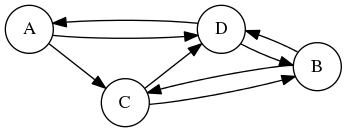
\includegraphics{tex/grafo_H2E6.png}
	\end{center}

Para ver el tiempo medio de retorno a A, podríamos estudiar las  probabilidades, pero es bastante lioso.

Como ya tenemos que es regular sabemos que es irreducible y podemos usar que:

\textit{Tiempo medio de retorno al estado $i$ = inverso de la i-ésima coordenada de la \textbf{distribución límite} = \textbf{única} distribución estacionaria. (es única porque es regular)}

Sabiendo esto calculamos la distribución estacionaria $$\begin{cases}
(\prod)P = (\prod)\\
(\prod) = (x,y,z,t)\\
\end{cases} \rightarrow \begin{cases}
\frac{t}{2} = x\\
\frac{z+t}{2} = y\\
\frac{x+y}{2} = z\\
\frac{x+y+z}{2} = t\\
x + y + z + t=1\\
\end{cases}$$

Y resolviendo este sistema queda que:
$$(\prod) = (x,y,z,t) = \left(\frac{1}{6}, \frac{5}{18} , \frac{2}{9}, \frac{1}{3}\right)$$

Por lo tanto el tiempo medio del primer retorno a A es : \textbf{6}.

Y fijándonos también en la distribución límite vemos que la página más "importante" es \textbf{D} , luego \textbf{B} , \textbf{C} y finalmente \textbf{A}.


% 	Vamos a ver las probabilidades que tenemos de %volver a $A$ para cada número de pasos $n$:
%	\[P_n(\text{ vuelta a A}) = \left\{ %\begin{array}{lcc}
 %            0 &   si  &  n=1\\
  %           \\ 1/4 &   si  &  n=2 \\
   %          \\ 1/8 &   si  &  n=3 \\
    %         \\ 2/16 &   si  &  n=4 \\
     %        \\ 2/32 &   si  &  n=5 \\
      %       \\ 4/64 &   si  &  n=6 \\
       %      \end{array}
   %\right.\]
  % En definitiva estamos teniendo
   %\[P_n = P\left(C \to D \text{ en } n-2 \text{ %pasos}\right) + P\left(D \to D= \text{ en } n-2 %\text{ pasos}\right)\]
   %Vamos a analizar esta probabilidades por separado

   %TO BE CONTINUED (creo que se lo que tiene que %salir, pero no veo clara la explicación %matemática)
   %\begin{itemize}
   %\item
   %\[P_n = P\left(C \to D \text{ en } n-2 \text{ %pasos}\right) \]

   %\item
   %\[ P\left(D \to D= \text{ en } n-2 \text{ %pasos}\right)\]
   %\end{itemize}
\end{problem}

\begin{problem}[7]
	Recuerda que el algoritmo \textit{page rank} sustituye la matriz de transición $P$ por $P_i = (1-ε)P+εE$ donde $E$ es la matríz $N\times N$ con todos sus elementos $1/N$. Explica por qué $P_i$ es una matriz de transición lícita de una cadena de Markov regular cuando $0 \leq t \leq 1$.
	\solution
	\textcolor{blue}{Hecho por Pedro. No fiarse al 100\%}

	Para empezar es evidente que, en caso de corresponderse con una cadena de Markov, $P_ε$ representaría una cadena de Markov regular, pues ella misma tiene todos sus elementos no nulos (tendríasmo $k=1$).

	Puesto que todas las filas de $P$ suman 1, tendremos que las filas de $P_i$ sumarán $1-ε+ε=1$, ya que los elementos de la matríz $E$ también suman 1.

\end{problem}

\begin{problem}[8]
	Consideramos tres páginas web A,B y C. Las dos últimas están enlazadas entre ellas y A enlaza a B. Comprueba que la distribución límite cuando se aplica el algoritmo \textit{page rank} viene dada por
	\[\left(\frac{ε}{3}, \frac{1-2ε/3}{2-ε}, \frac{1-ε+ε^2/3}{2-ε}\right)\]
	Halla autovalores de $P_i$ y con ellos trata de explicar cómo varía la ``velocidad'' de convergencia en términos de ε. Por ejemplo, ¿e bueno o malo coger el número de iteraciones como el inverso de ε?
	\solution

	La matriz de transición de este sistema, suponiendo que todos los enlaces tienen igual probabilidad de ser pulsados, es:
	\[P= \left( \begin{matrix}
	0&1&0\\
	0&0&1\\
	0&1&0\\
	\end{matrix}\right)\]

	La matríz $P_i$ empleada por el algoritmo de \textit{page rank} será de la forma
	$$P_{\epsilon} = (1-\epsilon) \cdot P + \epsilon \frac{1}{3} \left(
	\begin{matrix}
	1&1&1\\
	1&1&1\\
	1&1&1\\
	\end{matrix} \right)$$

	\[P_ε= \left( \begin{matrix}
	ε/3&1-2ε/3&ε/3\\
	ε/3&ε/3&1-2ε/3\\
	ε/3&1-2ε/3&ε/3\\
	\end{matrix}\right)\]

	Puesto que $P_ε$ tiene todos sus elementos no nulos, se trata de una cadena regular y por tanto su distribución límite coincide con la distribución estacionaria. Planteando las ecuaciones habituales para el cáculo de la distribución estacionaria obtenemos exactamente la distribución dada en el enunciado.

	Es decir, bastaría con resolver el sistema
	\[\vx P_ε=\vx\]


	En vez de hacer ese cálculo tal cual lo mejor es hacerlo por trozos.

	$$(\prod) P_{\epsilon} = \left(1-\epsilon\right)\left(\prod\right)P + \frac{\epsilon}{3} \left(\prod\right) \left(
	\begin{matrix}
	1&1&1\\
	1&1&1\\
	1&1&1\\
	\end{matrix} \right) = \left(\prod\right) $$

	Entonces:

	$$ (1-\epsilon)(0,x+z,y) + \frac{\epsilon}{3} (x + y + z) (1,1,1) = (x,y,z) $$

	Si a esta ecuación le añadimos que $ x + y + z = 1$ obtenemos el sistema:

	$$(1-\epsilon)(0,x+z,y) + \frac{\epsilon}{3} (1,1,1) = (x,y,z) \rightarrow \begin{cases}
	\frac{\epsilon}{3}= x\\
	(1-\epsilon)(x+z) + \frac{\epsilon}{3}=y\\
	(1-\epsilon) y + \frac{\epsilon}{3} = z\\
	x + y +z = 1
	\end{cases}$$

	y el resultado es:
	$$(x,y,z) = \left(\frac{ε}{3}, \frac{1-2ε/3}{2-ε}, \frac{1-ε+ε^2/3}{2-ε}\right)$$

	Para la parte de los \textbf{autovalores}:
	Podemos ver que los autovalores de esta matriz son $1,0,ε-1$ y sus autovectores:
	\[(1,1,1) \ \ \left( 1-\frac{3}{ε},1,1\right) \ \ \left(1,-\frac{-3+ε}{-3+2ε},1 \right)\]

	A la hora de estudiar la velocidad de convergencia, tenemos que el tiempo que tardará la matriz diagonal formada por los autovalores en estabilizarse cuando estamos calculando potencias.

	En este caso tenemos dos autovalores constantes e idempotentes por lo que todo depende del último autovalor: $ε-1$. Por tratarse de un número negativo (ε < 1) va a oscilar en torno al 0. Cuanto mayor sea ε más se acercará al 0 y las oscilaciones serán cada vez menores, por lo que convergerá más rápido.
\end{problem}

\begin{problem}[9]
	En una urna hay dos bolas blancas y otras dos negras. Escogemos dos al azar y las pasamos a otra urna. En cada instante se escoge al azar una bola de cada urna y se intercambian.

	Considerando los estados dados por el número de bolas negras en la primera urna más uno, escribe la matriz de probabilidades de transición y halla la distribución límite, probando que existe

	\solution

	Tenemos la matriz:
	\[P= \begin{pmatrix}
	0&1&0\\
	1/4&1/2&1/4\\
	0&1&0
	\end{pmatrix}\]
	La matriz indica que si no tenemos ninguna bola negra en la primera urna, la probabilidad de hacer el movimiento indicado y seguir sin bolas negras en esa urna es 0 ($p_{11}$). Si tenemos una bola negra, la probabilidad de seguir teniendo una bola negra es $p_{22}=1/2$ ya que podemos coger las dos blancas o las dos negras e intercambiarlas (dos de 4 opciones)

	Podemos ver a simple vista que el cuadrado de esa matríz tendrá todos sus elementos no nulos, por lo que la cadena de Markov que estamos trabajando es regular y por tanto existe distribución límite, que coincide con la distribución estacionaria.

	Procedamos pues a calcular esta distribución estacionaria, resolviendo el sistema $(x,y,z) P = (x,y,z)$:

	\[
	(x,y,z) \begin{pmatrix}
	0&1&0\\
	1/4&1/2&1/4\\
	0&1&0
	\end{pmatrix} = (x,y,z)
	\]

	Que nos da el siguiente sistema de ecuaciones:

	\[\begin{cases}
		 \frac{1}{4}y=x\\
		 x+\frac{1}{2}y+z=y\\
		 \frac{1}{4}y=z\\
		 x+y+z=1
	\end{cases} \implies x=z=\frac{1}{6}, y = \frac{2}{3}\]
\end{problem}

\begin{problem}[10]
Suponemos que variamos el esquema del ejercicio anterior considerando las 4 bolas negras y numeradas. En cada paso elegimos un número al azar y cambiamos de urna la bola correspondiente (sin reemplazarla). Halla la distribución estacionaria.
	\solution

	Aunque el enunciado dice que son numeradas, no lo hemos tenido en cuenta en clase, para no complicarlo demasiado.

	En esta ocasión, el estado $i$ representará la situación en que hay $i$ bolas en la primera caja (el elemento de la matriz $p_{02}$ representará la probabilidad de pasar de no tener ninguna bola a tener 2). Con esta consideración, la matriz de transición queda:

	\[P= \left( \begin{matrix}
	0&1&0&0&0\\
	1/4&0&3/4&0&0\\
	0&1/2&0&1/2&0\\
	0&0&3/4&0&1/4\\
	0&0&0&1&0\\
	\end{matrix}\right)\]

	Para buscar la solución estacionaria sólo tenemos que plantear el sistema de ecuaciones habitual:
	\[\vx P = \vx\]

	que, descompuesto en coordenadas, nos queda:

	\[\begin{cases}
		 a=\frac{1}{4}b\\
		 b= a+\frac{1}{2}c\\
		 c= \frac{3}{4} \left(b+d\right)\\
		 d= \frac{1}{2}c+e\\
		 e= \frac{1}{4}d\\
		 a+b+c+d+e=1
	\end{cases} \implies ... \implies (a,b,c,d,e) = \frac{1}{16} (1,4,6,4,1)\]


\end{problem}

\begin{problem}[11]
 Se lanza una moneda hasta que salga una de las secuencias XCC, CXC, CCX. ¿Por
cuál de ellas apostarías?

 Trata de formular el problema como una cadena de Markov (no irreducible) con estados $\{$XX, XC, CX, CC, XCC, CXC, CCX $\}$, donde los estados representan
las dos últimas tiradas o el fin del juego. Calcula el número de tiradas esperado del juego.
	\solution
	\textcolor{blue}{Hecho por Pedro. No fiarse al 100\%}

	La primera pregunta es fácil, lo óptimo sería apostar a la que no apuesten \textbf{Solar} ni \textbf{Cazakas}.

	La cadena de Markov de este ejercicio, con los estados indicados en el enunciado, sería:
	\begin{center}
	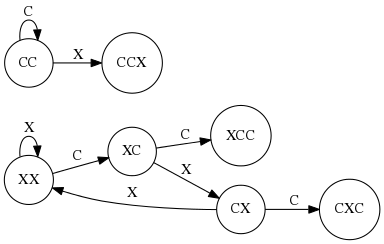
\includegraphics{tex/grafo_H2E11.png}
	\end{center}

	Tal y como nos adelantaba el enunciado, la cadena obtenida no es irreducible. No podemos ir de cualquier estado a cualquier otro en un número finito de pasos.

	TO BE CONTINUED...

	\textcolor{blue}{No se como formular lo que viene ahora correctamente.}

\end{problem}

\begin{problem}[12]
	Da un ejemplo de una cadena de Markov finita regular tal que $P^6$ temga algún ememento nulo, donde $P$ es la matriz de transición.
	\solution
	\textcolor{blue}{Hecho por Pedro. No fiarse al 100\%}

	Basta con escribir un ejemplo tan absurdo como una cadena lineal en la que $p_{ij}=1 \iff i+1=j$ y $P_{ij}=0$ en otro caso.

	Una cadena de este tipo, siempre que sea finita, será regular así que basta con hacerla con más de 6 nodos, de forma que no se pueda llegar del primer estado al último en 6 pasos, lo que provocaría un 0 en la matriz $P^6$.
\end{problem}

\begin{problem}[13]
	Consideramos la cadena de Markov finita con estados en $\ent$, consistente en que en $\ent^+$ damos un paso a la derecha con probabilidad 0.4 y a la izquierda con probabilidad 0.6, mientras que en $\ent^-$ estas probabilidades están intercambiadas. Además, desde el 0 se alcanzan el 1 y el -1 con probabilidad 1/2.

	Como el origen ``atrae'' a los otros estados, se puede probar que el tiempo medio de retorno es finito y la teoría asegura que existe una distribución estacionaria. ¿Cuál es? Por la simetría se puede suponer que toma los mismo valores en los negativos que en los positivos

	\solution
	\textcolor{blue}{Hecho por Pedro. No fiarse al 100\%}

	Aunque la idea sería la de siempre, en este caso el sistema de ecuaciones nos queda con infinitas ecuaciones.

	Vamos a restringirnos a los 2 primeros enteros positivos y negativos y el 0 y supondremos que para los que siguen la distribución será la misma que para los enteros 2 y 3.

	Para representarlo en forma de matriz, consideramos que en los extremenos tenemos tantas posibilidades de quedarnos fijos como posiblidades habría de llegar a esos valores desde estados que quedan excluídos de nuestra simplifiación menos las probabilidades que había de salir de nuestra simplifiación.

	Podemos suponer, sin demasiado riesgo de equivocarnos, que en la distribución estacionaria tendremos los mismos valores en todos los enteros con valor absoluto mayor o igual que 2.

	Por tanto, siendo $a,b,c,d,e$ los valores de los estados $-2,-1,0,1,2$ respectivamente, simulando un movimiento y forzando la estacionalidad de esa solución, tendremos:
	\[\begin{cases}
		a = 0.6a+0.4b\\
		b = 0.6a+0.5c\\
		c = 0.6b+0.6d\\
		d = 0.5c+0.6e\\
		e = 0.4d+0.6e\\
	\end{cases} \implies \begin{cases}
		a = b \\
		0.4 b =0.5c \\
		c = 0.6b+0.6d\\
		0.4d = 0.5c \\
		e = d
	\end{cases} \implies a=b=c=d \ c = 1.2a\]

	De modo que habría infinitas distribuciones estacionarias, que serían todas aquellas que cumplen esa relación:
	\[\left(a,a,1.2a,a,a\right)\]

\end{problem}

\begin{problem}[14]
	El número total de partículas se conserva a lo largo del tiempo en el modelo discretizado de movimiento browniano (paseo aleatorio) en una dimensión. Traduce esto en alguna ley de conservación para le ecuación del calor en $\real$ (con dato de decaimiento rápido) y demuéstrala
	\solution

	\textcolor{blue}{Hecho por Pedro. No fiarse al 100\%}

	El movimiento browniando en una dimensión se corresponde con el análisis del sistema:

	\begin{center}
	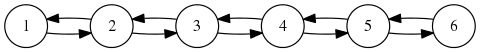
\includegraphics{tex/browniano_1_dim.png}
	\end{center}
	imaginando que se extendiera hasta el infinito por los laterales.

	Consideramos que la probabilidad de coger cualquiera de los dos caminos que parten de un grafo es la misma, de modo que
	\[\prob{X_{n+1}=j}=\frac{1}{2}\prob{X_n = j-1}+\frac{1}{2}\prob{X_n=j+1}\]

	Establezcamos que los valores de tiempo son 0, 1h, 2h, ... y que una partícula se mueve saltando entre los puntos de $ε\ent$ (representados por los nodos de nuestro grafo). Consideramos $S=\ent$ y $X_n$ será la variable aleatoria que toma el valor $j$ cuando la partícula está en la posición $εj$ en tiempo $hn$.

	Como vimos en clase, el análisis combinatorio bien conocido del \textit{paseo aleatorio} unidimensional muestra que, con esta notación, en tiempo $hn=1$ la partícula se aleja del origen del orden de $ε\sqrt{n}$.

	Puesto que queremos que en $hn=1$ la distancia se mantenga acotada, deberámos tomar $h=ε^2/2$\footnote{Consiguiendo que la distancia al origen sea $ε\sqrt{n}=ε\sqrt{\frac{2}{ε^2}} = \sqrt{2}$, que es constante}. Nuestro objetivo será estudiar qué ocurre cuando $ε \to 0$.

	Una vez aclarado esto podemos escribir:
	\[\frac{\prob{X_{n+1}=j}-\prob{X_n=j}}{h}=\frac{\prob{X_n=j-1}+\prob{X_n=j+1}-2\prob{X_n=j}}{ε^2}\]

	Puede comprobarse que la igualdad es cierta de forma sencilla basándose en la relación: $1/2=hε^2$.

	Esperamos que cuando $ε\to 0$, $\prob{X_n=j}$ pueda expresarse como una función buena, que dependa del espacio y el tiempo, $u(x,t)$ con $x=jε$ y $t=hn$. De esta forma la ecuación anterior conduce a:
	\[\frac{u(x,t+h)-u(x,t)}{h}=\frac{u(x-ε,t)+u(x+ε,t)-2u(x,t)}{ε^2}\]
	y podemos observar de manera trivial que esta ecuacuión se corresponde con:
	\[\frac{\partial u}{\partial t}=\frac{\partial^2u}{\partial x^2} \ x \in \real, \ t > 0\]

	Y esta última ecuación no es otra que la \textbf{ecuación del calor}

\end{problem}

\begin{problem}[15]
	Paseamos por $\ent^2$ partiendo del origen y avanzando de uno en uno en una dirección: N, S, E, O, elegida al azar. Demuestra que el número de retornos al origen en a lo más 2M pasos es en media:
	\[\sum_{n=1}^M 4^{-2n}\sum_{k+l=n}(2n)!/(k!)^2(l!)^2\]
	Comprueba que esta serie diverge cuando $M \to \infty$, expresando la suma interior como
	\[4^{n-1}π^{-2}\int_{-π}^π\int_{-π}^π\left(\sin(x)+\sin(y)\right)^{2n}dxdy\]
	\solution


\end{problem}
